    \subsection{Server Side}\label{Server Side Design}

    In this chapter we are going to introduce the design, configuration and modification that we are going to do on the server side. In section \ref{Server Introduction} we will introduce the framework that we have built upon and what we are going to do with it. Next follows use cases, \ref{Server Use Cases}. Section \ref{Description of ESB concepts} will go into more detail about what the framework consists of. The section will also guide you through the basic processing units which is used in the framework. The next section, \ref{Textual Server Dataflow}, contains the dataflow through the server side, which will help you get a good overview of our thoughts about the design. \ref{Extensions to the ESB} goes into detail in describing our custom components in the framework, and together with the dataflow should give you a good understanding of the whole server side. Together with section \ref{Server Sequence Diagrams} you should get good system overview. Section \ref{Configuration of the ESB} will give you the details about how we have configured the framework, it will not contain description of how we have set variables during testing, but using this description should make it possible to get the framework up and running. The last section, \ref{Modification of the ESB} will depict how we have modified the framework to be able to meet our requirements, with this section you should be able to tell what modifications were needed and how we have altered those pieces. 

    \subsubsection{Introduction}\label{Server Introduction}
    The server side architecture consists of several components, the WSO2 ESB, the WSO2 Identity Server (IS) the Monitoring Service and the GlassFish server. The GlassFish server is not necessary to modify, the MS is something we must assume exist in the network, and in the IS we only have to configure it to work with the ESB. The ESB is what we have to modify, configure and extend to meet the requirements set.

    The ESB will be used to implement QoS for the web services. To do this, it will have to communicate with the IS and the MS, in addition to the clients and the services. The ESB must be configured to work as a proxy for the services on the GlassFish server, and the IS. It will also be configured to use certain mediation sequences for incoming requests and outgoing responses. The extensions to the ESB consists mainly of custom mediators used in the mediation sequences. These mediators will have the tasks of determining priority of messages, contacting the MS for bandwidth data, and enforcing the priority. There will also be made modifications to the ESB source code to allow for setting the diffserv field in the IP header.
    
    \subsubsection{Use Cases}\label{Server Use Cases}
    This section will outline the use cases that we have thought of in relation to the server side. With the help of these you should get a rough idea of what we want the server side to be able to do.\\\\
    \textbf{Title:} Request for SAML authentication \\
    \textbf{Actors:} Client, Enterprise service bus(ESB) and Identity server(IS)\\
    \textbf{Main}
    \begin{enumerate}
        \item Client sends a SOAP message to ESB containing credentials
        \item ESB mediates the message to the IS
        \item IS fetches SAML Token
        \item IS sends the message to ESB
        \item ESB adds metadata to SOAP message
        \item ESB sends the message back to the client
    \end{enumerate}
    \textbf{Extensions:}
    \begin{itemize}
        \item[] 3a. Invalid credentials 
        \item[] 4a. IS returns error message
        \item[] 6a. ESB sends error message to client
    \end{itemize}
    \textbf{Precondition:}
    \begin{itemize}
        \item There exists a connection between the client and the ESB
    \end{itemize}
    \\
    \textbf{Title:} Request mediation\\
    \textbf{Actors:} Client, ESB, GlassFish\\
    \textbf{Main}
    \begin{enumerate}
        \item Client sends SOAP message with SAML Token to ESB proxy
        \item ESB authenticates SAML Token(See Authentication use case)
        \item ESB removes SAML metadata from message
        \item ESB adds metadata to message context.
        \item ESB sends message to GlassFish endpoint
    \end{enumerate}
    \textbf{Extensions:}
    \begin{itemize}
        \item[] 2a. SAML Token is invalid
        \item[] 2b. ESB sends error message to client
    \end{itemize}
    \textbf{Precondition:}
    \begin{itemize}
        \item Client is connected to ESB
    \end{itemize}
    \\
    \textbf{Title:} Response mediation \\
    \textbf{Actors:} Client, ESB, GlassFish \\
    \textbf{Main}
    \begin{enumerate}
        \item GlassFish sends message to ESB
        \item ESB sets priority metadata in message context and SOAP header.
        \item ESB retrieves bandwidth information (See Monitoring Service communication use case)
        \item ESB prioritizes message (See Prioritize message use case)
        \item ESB sends message to Client
    \end{enumerate}
    \textbf{Extensions:} \\
    \textbf{Precondition:}
    \begin{itemize}
        \item Request mediation
    \end{itemize}
    \\
    \textbf{Title:} Monitoring Service communication\\
    \textbf{Actors:} Monitoring Service(MS), ESB\\
    \textbf{Main}
    \begin{enumerate}
        \item ESB requests bandwidth information from MS to a specific address
        \item MS returns bottleneck bandwidth to the ESB, as well as the address of the last Tactical Router before the endpoint.
    \end{enumerate}
    \textbf{Extensions:}
    \begin{itemize}
        \item[]	1a. ESB specifies an invalid address
        \item[]	2a. MS returns no information
        \item[]	2b. Address is in the same sub net as the ESB
    \end{itemize}
    \textbf{Precondition:}
    \begin{itemize}
        \item Response mediation
    \end{itemize}
    \\
    \textbf{Title:} Prioritize messages\\
    \textbf{Actors:} ESB\\
    \textbf{Main}
    \begin{enumerate}
        \item ESB acquires QoS information (by magick)
        \item ESB adds QoS information to the SOAP header of the message
        \item ESB sets diffserv field in IP header
    \end{enumerate}
    \textbf{Extensions:}\\
    \textbf{Precondition:}
    \begin{itemize}
        \item Response mediation
        \item Monitoring Service communication
    \end{itemize}
    \\
    \textbf{Title:} Authenticate SAML token\\
    \textbf{Actors:} ESB, IS\\
    \textbf{Main}
    \begin{enumerate}
        \item ESB sends SAML token to IS
        \item IS authenticates the token
        \item IS sends verification to ESB
    \end{enumerate}
    \textbf{Extensions:}
    \begin{itemize}
        \item[]	2a. SAML token is not valid.
        \item[]	3a. IS sends error to ESB
    \end{itemize}
    \textbf{Precondition:}
    \begin{itemize}
        \item Request Mediation
    \end{itemize}

    \subsubsection{Description of ESB concepts}\label{Description of ESB concepts} 

    In this section we will shortly describe some important concepts of the ESB and message mediation.

    A mediator is the basic processing unit in \gls{synapse}\footnote{An enterprise service bus}. Each message going through the ESB gets mediated through a sequence of mediators, which can be configured through either XML or WSO2’s graphical user interface. As long as the mediator inherit from a Synapse interface, any custom mediator can be used in the same manner as the built in mediators. To control the flow of messages through the ESB, there are two paths that can be controlled, the “in sequence” and the “out sequence”, which can also be configured to only apply for certain endpoints.

    The ESB is built around the notion of a message context, this object contains all the information regarding the message and the context around it. In the message context we can add properties, manipulate the message itself and manipulate the sending streams of the message. All the properties added during the receiving of a message is also added to the outgoing message, which we can use to our advantage.

    Each mediator in the sequence get access to the message context of the incoming or the outgoing message and can thus manipulate the context to its liking. When the mediator is done with the work it is supposed to do, it either calls the next mediator, sending it the possibly altered message context or returning true to indicate that the work is done.

    \subsubsection{Dataflow}\label{Textual Server Dataflow} 
        This section describes the data flow through the ESB with the help of two diagrams. As a bonus, these diagrams show the general architecture of the server side very well.
\\
        \begin{figure}[h]
            \centering
            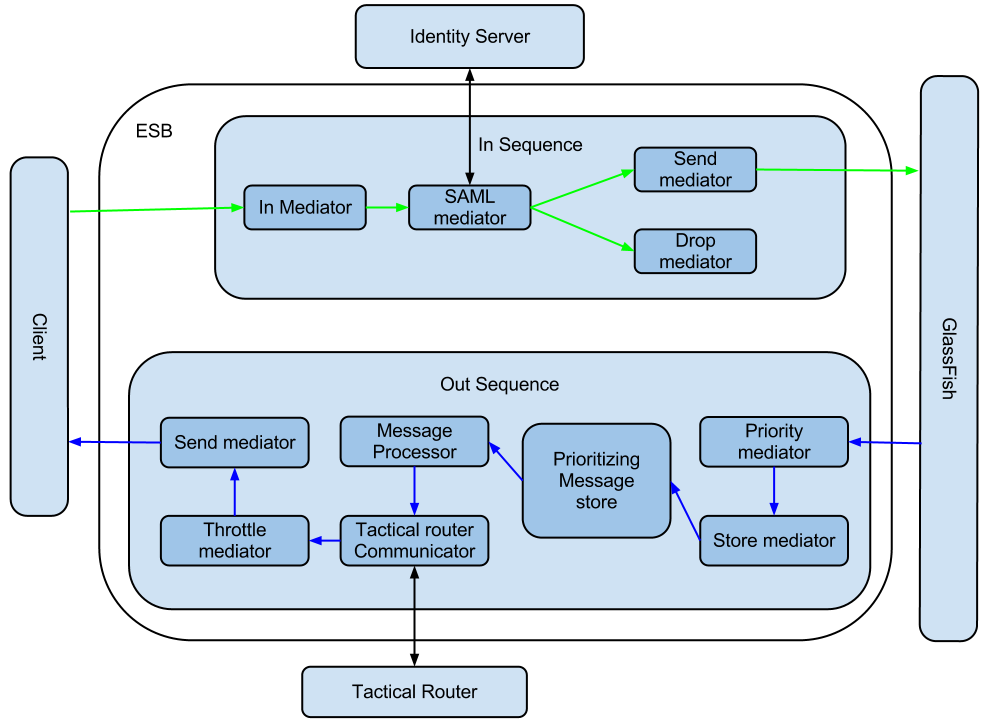
\includegraphics[scale=0.4]{DataFlowDiagramServer}
            \caption{Server Data Flow}
            \label{fig:DataFlowDiagramServer}
        \end{figure}
\\
Service Request :\\
To follow this flow, follow the green arrows in figure \ref{fig:DataFlowDiagramServer}. The ESB receives a request message from a Client, it is then authenticated or, if not, an error is sent back to the client. If it is not authenticated the flow stops, otherwise the message is sent to the SAML mediator, and then to the send mediator which sends it to the service endpoint on the GlassFish server, and the flow is over.
\\\\
Service Response:\\
To follow this flow, follow the blue arrows in figure \ref{fig:DataFlowDiagramServer}. The ESB receives a response message from the Service, it is then sent through a sequence of mediators, first the Metadata mediator, and then  the Store mediator. The Store mediator stores the message in the Prioritized Message Store. The message is stored until the Sampling Message Processor picks it out before sending it on to another sequence of mediators. First in the sequence is the MS mediator, then the Throttle Mediator and finally the Send mediator. The send mediator sends the message back to the client and the flow is completed.
\\
    \begin{figure}[h]
        \centering
        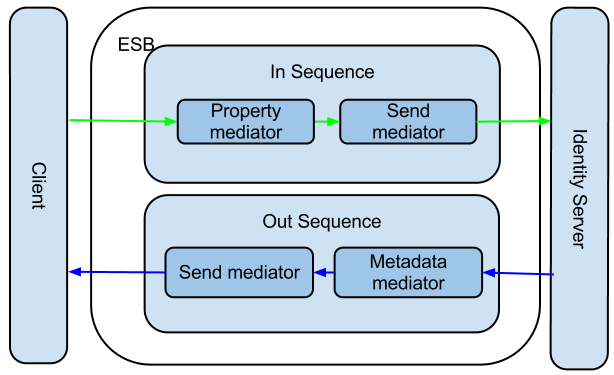
\includegraphics[scale=0.5]{SAMLauthenticationflow}
        \caption{SAML Authentication Flow}
        \label{fig:SAMLauthenticationflow}
    \end{figure}
\\           
SAML Authentication Request:\\
The ESB receives a request (from a Client) directed at the Identity Server (IS), the ESB relays this message to the IS. The ESB receives the response from the IS, and sends it through a mediator sequence consisting of the Priority mediator and the Send mediator. The send mediator sends the response to the Client.

    \subsubsection{Extensions to the ESB}\label{Extensions to the ESB} 
    This section will contain a textual description of all the mediators used in the ESB. First we will describe all the custom mediators and extensions we make to the ESB, and then a short description of the built-in mediators we will use.
\\\\
\textbf{Custom mediators:}\\\\
SAML mediator:\\
    This mediator retrieves the user role from the SAML authentication and set this as a property in the message context. The service is retrieved from the endpoint reference and set as another property.
\\\\
SendBack mediator:\\
    This mediator sends a SAML authentication error message back to the client. After the error is sent to the client, the message is forwarded to the Drop mediator. We are not quite sure if this mediator is needed or not, as it is difficult to determine this before having at least some other parts of the system ready for testing.
\\\\
Metadata mediator:\\
    This mediator retrieves the client role and service properties from the message context. These properties are then used along with a persistent registry to infer a priority for the message, and what the diffserv field in the IP header should be set as. The priority and diffserv values are then set as new properties in the message context.
    The diffserv property in the message context will be used in the synapse core to set the diffserv field before sending the message (See \ref{Modification of the ESB}).
\\\\
Prioritized Message store:\\
    This is not a mediator, but it is an important part of the response mediation sequence. This is a message store that stores messages in a priority queue. The queue is mainly ordered by the priority property of the message context, and secondly by the time when added. When retrieving messages from this store, the message on the top of the queue is returned. This ensures that high priority messages are processed before lower priority messages.
\\\\
MS mediator:\\
    This mediator retrieves the \gls{ipaddress}\footnote{A numerical label assigned to each device connected to the Internet} of the receiving client from the endpoint reference in the message context. It sends this IP address to the Monitoring Service and gets the IP address of the last Tactical Router on the path to the client, as well as the limiting bandwidth on the path. The mediator then sets this information as properties in the message context before sending the message to the next mediator.
\\\\
Throttle mediator:\\
    This mediator is used to ensure that high priority messages are sent first, by disrupting already sending messages, and it tries to ensure that the network is not being overflowed by this server by holding back messages. To determine what to disrupt and what to hold back, and for how long, several properties are used; the priority of the message, the available bandwidth, the IP address of the client side Tactical Router, and the real time demand of the request. In order to do this, the mediator must keep a list of sending messages and where those messages are going. This mediator does not have a companion sequence diagram as of the midterm report. The reason behind this is currently a lack of possibility to test the mediator, this will however be remedied when we start to implement the mediators. Once we are more sure of what this mediator will be capable of, we will make a sequence diagram for it.
\\\\
\textbf{Built in Mediators:}\\\\
Drop mediator:\\
    This is a built in mediator that drops the message, preventing further processing.
\\\\
Send mediator:\\
    This is a built in mediator that sends the message to an endpoint (the requested service).
\\\\
Store mediator:\\
    This is a build in mediator that stores the message context in a message store, here this is the Prioritized Message store.
\\\\
Sampling Message Processor:\\
    This is not a mediator. It is a built in class that takes messages out of the Prioritized Message Store at a defined interval. And then sends them to a mediator sequence, here starting with MS mediator.

    \subsubsection{Sequence Diagrams}\label{Server Sequence Diagrams}
    This section contains some sequence diagrams which you can use to get a more in depth look into the code and methods used in the mediators above.
    
        \begin{figure}[H]
            \centering
            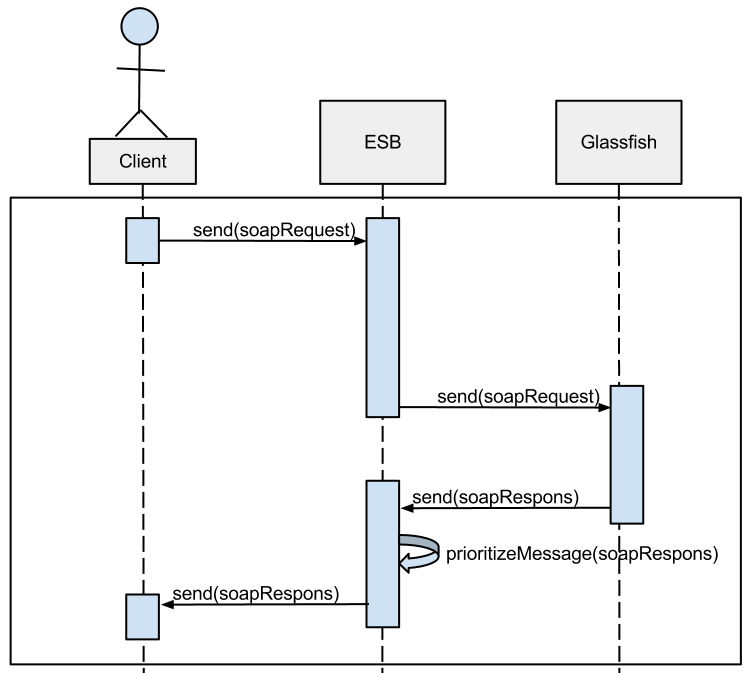
\includegraphics[scale=0.3]{System-levelsequencediagram}
            \caption{System-level sequence diagram}
            This high level diagram shows how the client communicates with web services through the ESB.
            \label{fig:System-levelsequencediagram}
        \end{figure}
        
        \begin{figure}[H]
            \centering
            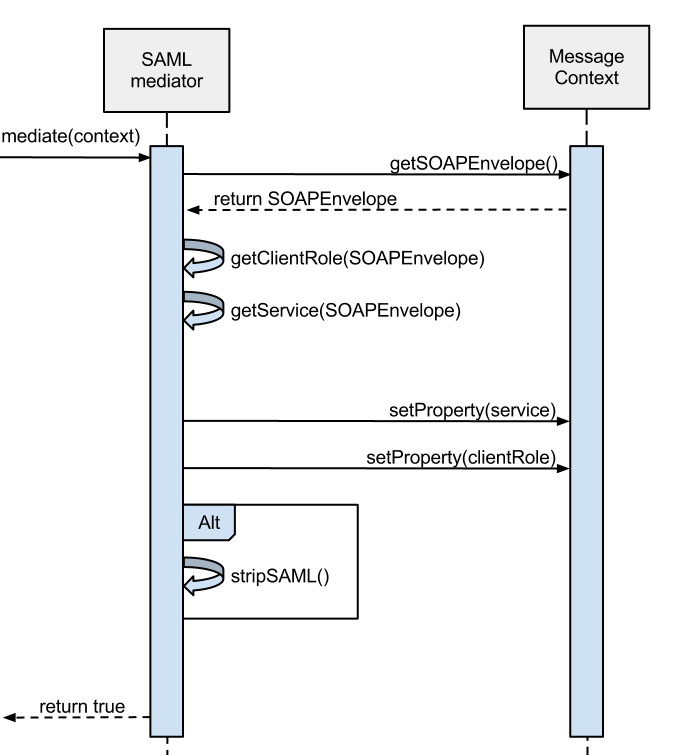
\includegraphics[scale=0.3]{SAMLmediator}
            \caption{SAML mediator sequence diagram}
            This diagram describes how the SAML mediator will get data from the message, and set it in the message context so it can be used later in the response sequence
            \label{fig:SAMLmediator}
        \end{figure}
        
        \begin{figure}[H]
            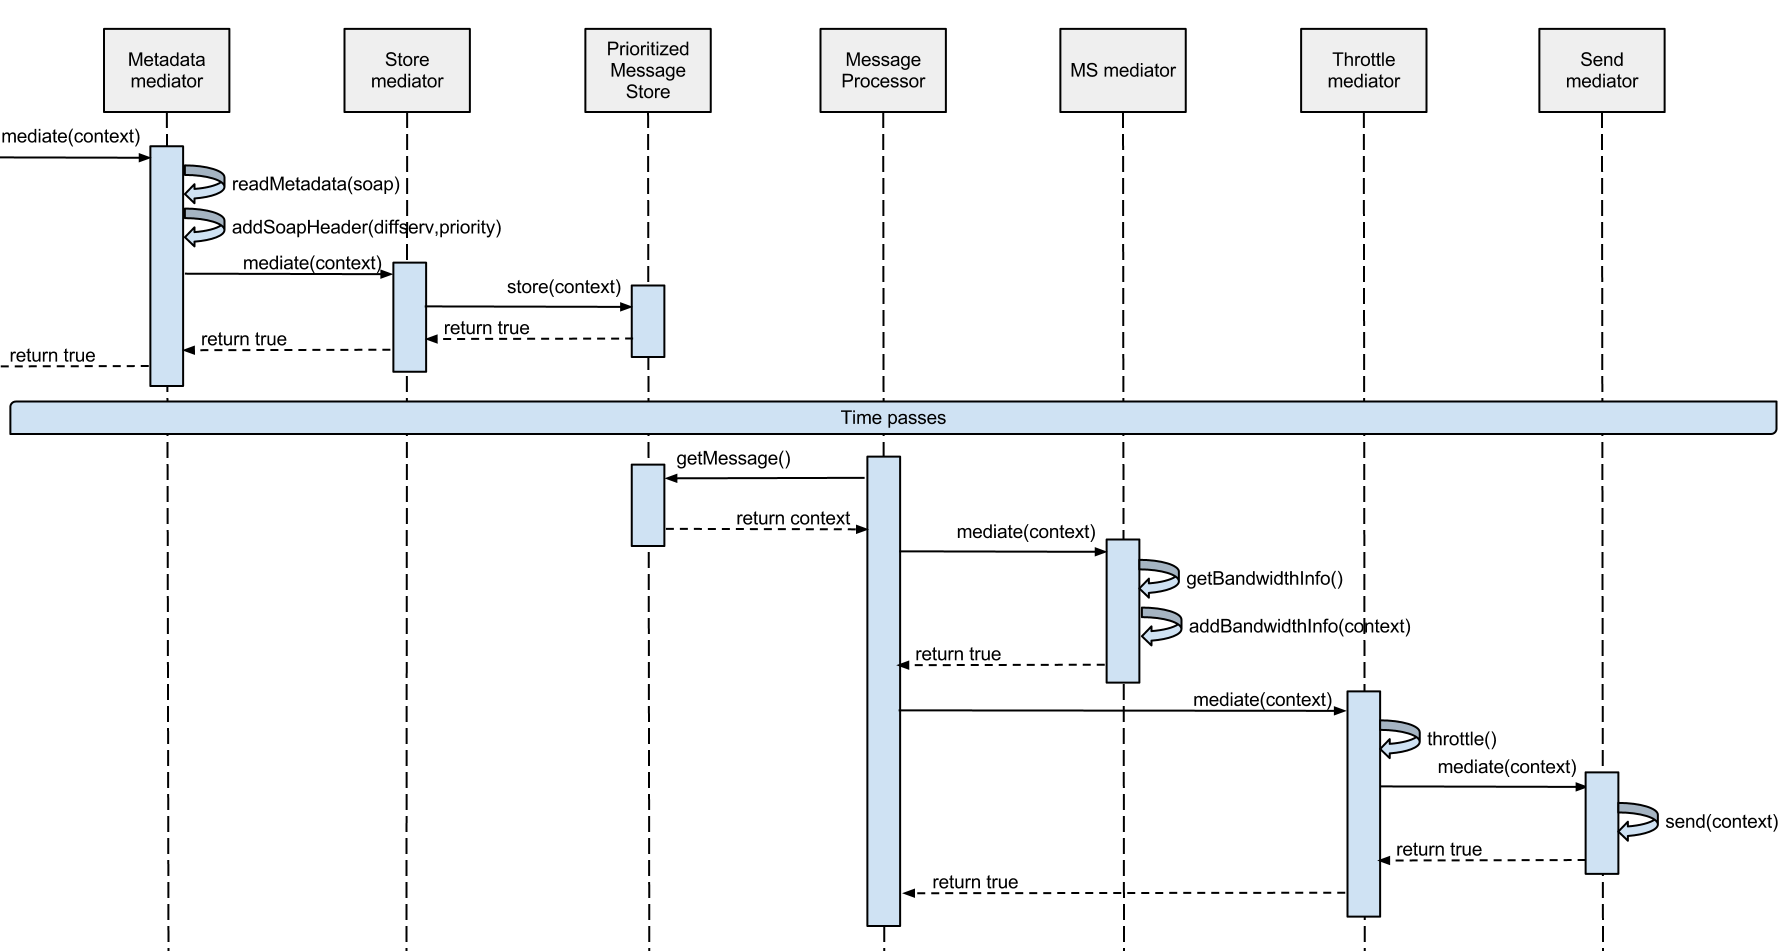
\includegraphics[scale=0.28,angle=-90]{Responsesequencediagram}
            \caption{Response sequence sequence diagram}
            This diagram describes, in some detail, how a response message from the web service to the Client is passed through the ESB.
            \label{fig:Responsesequencediagram}
        \end{figure}
    
        \begin{figure}[H]
            \centering
            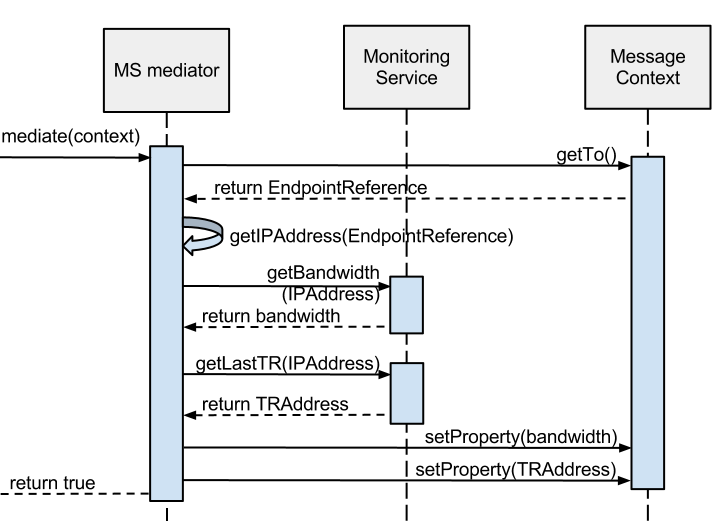
\includegraphics[scale=0.3]{MSmediatorsequence}
            \caption{Metadata mediator sequence}
            This diagram describes how the Metadata mediator retrieves previously stored properties from the message context, determines a priority for the message, and sets priority and diffserv properties in the message context
            \label{fig:MSmediatorsequence}
        \end{figure}
        
        \begin{figure}[H]
            \centering
            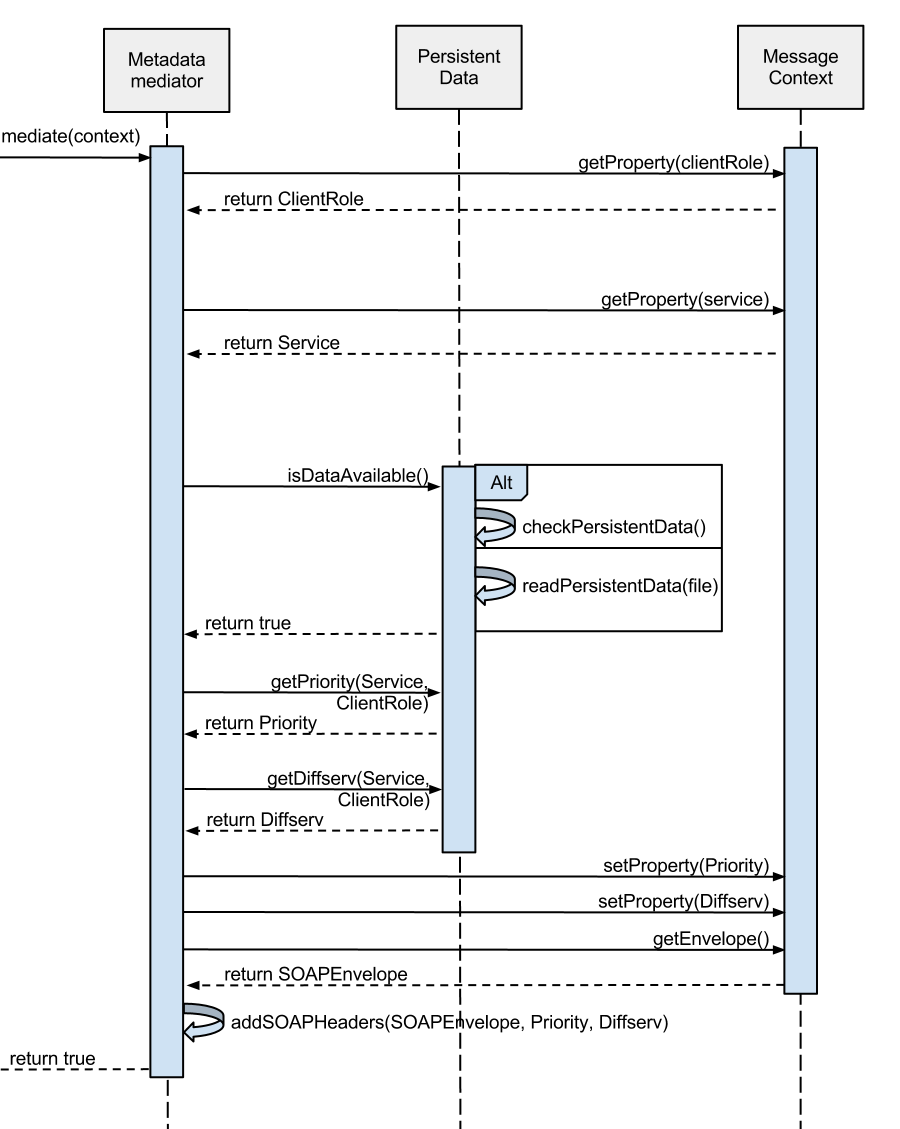
\includegraphics[scale=0.4]{Metadatamediatorsequencediagram}
            \caption{MS mediator sequence diagram}
            This diagram describes the MS mediator contacting the Monitoring Service for bandwidth information
            \label{fig:Metadatamediatorsequencediagram}
        \end{figure}

    \subsubsection{Configuration of the ESB}\label{Configuration of the ESB} 
    This section will be about how the ESB is to be configured.

    \subsubsection{Modification of the ESB}\label{Modification of the ESB} 
		The WSO2 ESB source code will have to be modified to allow for setting the diffserv field in the IP-header of packets sent. The idea is that we will set a property, DiffServ, in the message context, and let the HTTPsender get this property and set it on the socket used for sending.

The source code for all the dependencies of WSO2 ESB is included in its source code. As such we only altered files in this source. This made it easier for us to build and create a runnable instance of WSO2’s ESB. To also try and support future versions of Apache Synapse and WSO2 we have also applied the changes to the latest version of the underlying libraries.

In Apache Synapse we have altered the way it sends responses to already established connections. This alteration is dependent on support in the underlying library of Apache HTTPComponents(HC for short) which we have also altered to include support for setting traffic class. Since Synapse is dependent on HC we are, as of the midterm report, trying to get our changes accepted into HC\footnote{Link to our ticket in HTTPComponents HTTPCore issue tracker  [\href{https://issues.apache.org/jira/browse/HTTPCORE-295}{JIRA: HTTPCore Issue 295}]}. We have included in our references SVN diff files and included instructions on how to apply them to a newly downloaded version of HC. We are planning to also push our changes in Synapse upstream, but we are waiting for the acceptance of our HC changes first.
    
